The first lecture gives an introductory to RMT. Covering aome basic concepts in this topic. Most of the materials here are from the lecture notes \cite{eynardRandomMatrices2018}. 

\subsection{Motivation and Definiton of RMT}

\subsubsection{Physical Motivation of RMT}

A physical motivation is the study of Wigner on the topic of Spectrum of heavy neuleus. As an observable he studied the distribution of distance between the energy levels. We can define a observable as:
\begin{align}
  P(s) = \text{ statistical distribution of the distance s between neighbouring energy levels.}
\end{align}
or $ P(s)ds $ is the probability of picking out a pair of neighbourhood energy level that the distance between two neibourhood energy levels is between $ s $ and $ s + ds $.

The experimental result of this observable gives the following distribution:
\thm{
  Wigner Surmise 
\begin{align}
  P(s)=C_\beta s^\beta e^{-a_\beta s^2} \quad \beta\in\{1,2,4\}
\end{align}
}
Theoretically, this turns out to be the result when the Hamiltonian is a random matrix! Thus, it is interesting to study a theory of random matrix as Hamiltonian.


\subsubsection{Definition of RMT}

We define a random matrix model with a partition function:
\defi{
  Partition Function of Random Matrix Model
  
  For a Theory of $ N \times N $
  \begin{align}
    \mathcal{Z} = \int dM e^{-N \tr V(M)}
  \end{align}
where $ V(M) $ is a potential function of the matrix $ M $. The measure $ dM $ is defined as:
\begin{align}
  dM = \prod_{ij} dM_{ij}
\end{align}
}
There are different ensembles that one may be considering. For example, GUE defined as the ensemble of Hermitian matrices with potential $ V(M) = \frac{1}{2}M^2 $. We then may use Hermitian matrix ensemble as an example to study, yet some of the properties may be generalized to other ensembles. For Hermite matrices, the measure can be written as:
\begin{align}
  dM = \prod_i dM_{ii} \prod_{i<j} d(M_{ij}) d(M_{ij})^*
\end{align}

\subsection{Eigenvalue Decomposition}

To study a random matrix ensemble of real eigenvalues, eg, Hermite matrix ensemble, or real symmetric matrix ensemble, it is often useful to do an eigenvalue decomposition of the matrix $ M $. 

\subsubsection{Eigenvalue Decomposition of Hermite Matrix}

For a random ensemble of Hermite matrix $ M $, we can do an eigenvalue decomposition:
\begin{align}
  M = U^\dagger \Lambda U, \quad \Lambda = \text{diag}(\lambda_1, \lambda_2, \cdots, \lambda_N)
\end{align}
In this case, the measure can be written as:
\begin{align}
  dM = \Delta(\{\lambda_i\})^2  \prod_{i=1}^N d\lambda_i dU_{haar}
\end{align}
where $ dU_{haar} $ is the Haar measure of unitary matrix $ U $, and $ \Delta(\{\lambda_i\}) $ is the Vandermonde determinant:
\begin{align}
  \Delta(\{\lambda_i\}) = \prod_{i<j} (\lambda_i - \lambda_j)
\end{align}
Normally, we integrate out the angular part $ U $, integrate it out and get a suitable normalization.
\YL{[need an appendix to derive this and define the Haar measure.]}

\subsubsection{Effective Action}

Thus, in terms of the eigenvalues, the partition function can be written as a intergral over N parameters with an effective action:
\begin{align}
  \mathcal{Z} &= \int dM e^{-N \tr V(M)} = \int \prod_{i=1}^N d\lambda_i \Delta(\{\lambda_i\})^2 e^{-N \sum_{i=1}^N V(\lambda_i)} 
  &= \int \prod_{i=1}^N d\lambda_i e^{- N^2 I_{\text{eff}}(\{\lambda_i\})}
\end{align}
where the effective action is:
\begin{align}
  I_{\text{eff}}(\{\lambda_i\}) = \displaystyle\frac{1}{N} \sum_{i=1}^N V(\lambda_i) - \displaystyle\frac{1}{N^2} \sum_{i<j} \log(|\lambda_i - \lambda_j|)^2
\end{align}


\subsection{Resolvent and Density of States}

There are two important observables in RMT, and the study of the observables often lead to physical results. First we shall define the expectation value of an observable $ O(M) $ as:
\begin{align}
  \langle O(M) \rangle = \displaystyle\frac{\int dM O(M) e^{-N \tr V(M)}}{\int dM e^{-N \tr V(M)}} = \displaystyle\frac{1}{\mathcal{Z}} \int dM O(M) e^{-N \tr V(M)}
\end{align}

\subsubsection{Density of States}

The density of states is defined as:
\defi{
  Density of States $ \rho(x) $ for a give random matrix $ M $ with eigenvalues $ \{\lambda_i\} $ is defined as:
  \begin{align}
    \rho(x) = \displaystyle\frac{1}{N} \langle \sum_{i=1}^N \delta(x - \lambda_i) \rangle 
  \end{align}
}
We can understand it as a function probing the point of the eigenvalues on the real line. 
The expectation value of the density of states is then:
\begin{align}
  \bar{\rho}(x) = \langle \rho(x) \rangle = \displaystyle\frac{1}{N} \left\langle \sum_{i=1}^N \delta(x - \lambda_i) \right\rangle
\end{align}
In fact the effective action can be written in terms of the density of states as:
\begin{align}
  I_{\text{eff}}(\rho) \sim \int dx \rho(x) V(x) - \iint dx dy \rho(x) \rho(y) \log|x-y|^2
\end{align}
I write $ \sim $ because it is not rigorous and needs further regularization. 
\rmk{
  From now on, when saying the density of states $ \rho(x) $, we often mean the expectation value $ \bar{\rho}(x) $ unless otherwise specified.
}

\subsubsection{Resolvent}

The resolvent is defined as:
\defi{
  Resolvent $ W(z) $ for a given random matrix $ M $ with eigenvalues $ \{\lambda_i\} $ is defined as:
  \begin{align}
    W(z) = \displaystyle\frac{1}{N} \langle \tr \displaystyle\frac{{1}}{z - M} \rangle  = \displaystyle\frac{1}{N} \langle \sum_{i=1}^N \displaystyle\frac{1}{z - \lambda_i} \rangle
  \end{align} 
}
Note that we use $ z $ as a complec variable here, for we will be analytically continuing it to the complex plane. and it is naturally defined to be an average over the ensemble. 
There is an important relation between the resolvent and the density of states. We know that we have:
\begin{align}
W(x) = \int_{supp \rho} dy \displaystyle\frac{\bar{\rho}(y)}{x - y}
\end{align}
where $ supp \rho $ is the all the region where the density of states is non-zero for real $ y $. Thus it is an integral on the real axis. In an random ensemble, we know that we integrate over all possible Hermite matrices, with all possible eigenvalues on the real line. Thus $ supp \rho $ is given by covering a branch cuts of the resolvent on the real line. 

As an inverse of the above equation, we can write the density of states on the real line point $ x $ with the discontinuity of the resolvent across the branch cut at $ x $:
\begin{align}
  \bar{\rho}(x) = -\displaystyle\frac{1}{2\pi i} \left( W(x + i\epsilon) - W(x - i\epsilon) \right)
\end{align}
This can be proved by using the Sokhotski–Plemelj theorem:
\begin{align}
  \lim_{\epsilon\to 0^+} \displaystyle\frac{1}{x - y \pm i\epsilon} = \mathcal{P}\displaystyle\frac{1}{x - y} \mp i\pi \delta(x - y)
\end{align}
In fact if we inverse the relation we can get:
\begin{align}
  \rho(x)=-\frac{1}{\pi}\mathrm{Im}W(x)
\end{align}
which is powerful when we calculate the density of states from the resolvent.


\subsection{Columb Gas and Saddle Point}


\subsubsection{Large N and Columb Gas Saddle Point}

This effective action can be understood as a system of particles in 1 dimension with a external potential and a pairwise repulsive interaction. The external potential is given by $ V(\lambda) $, while the pairwise interaction is given by a 2D Coulomb interaction $ -\log(|\lambda_i - \lambda_j|) $.

If we consider the \textbf{Large N Limit} of the matrix model. The eigen values tend to stay in the minimal energy point yet the repulsive interaction prevents them from collapsing to a single point. This is often called the Columb gas picture of RMT.
\begin{figure}[H]
  \centering
  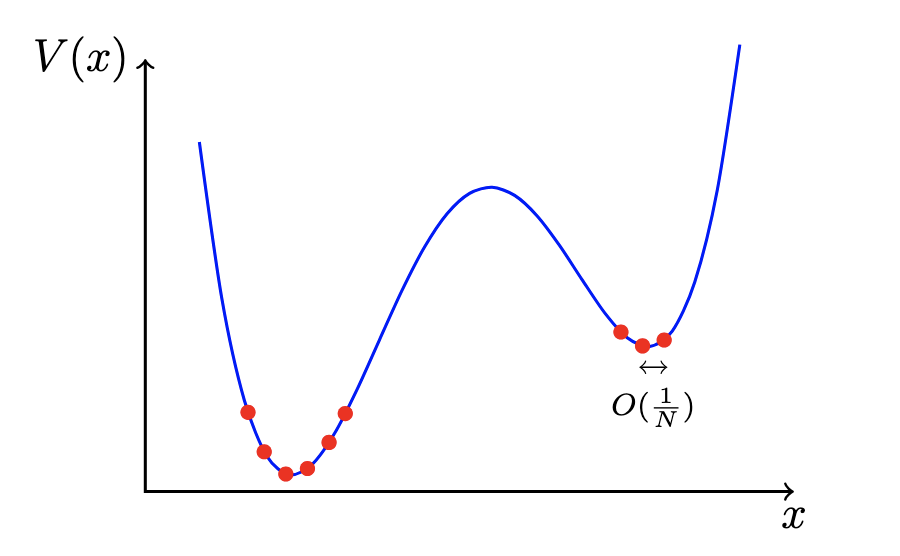
\includegraphics[width=0.4\textwidth]{assets/saddlepoint.png}
  \caption{Saddle Point of Columb Gas}
  \label{fig:saddlepoint}
\end{figure}

We first want to find the saddle point of this effective action. Varying the effective action with respect to $ \lambda_i $, we have:
\begin{align}
  \displaystyle\frac{\partial I_{eff}}{\partial \lambda_i} = 0 \quad \Rightarrow \quad V'(\lambda_i) = \displaystyle\frac{2}{N} \sum_{j\neq i} \displaystyle\frac{1}{\lambda_i - \lambda_j}
\end{align}
Given $ V(x) $ function this set of equations have finite solutions $ \{\lambda_i^{(0)}\} $. 

\subsubsection{Riccati equation}

We can then derive a relation between the resolvent and the potential. By studying the resolvent, we can derive an important equation called the Riccati equation. This equation related the resolvent to the potential function $ V(x) $ at the saddle point. 

When we consider the large $ N $ limit, we can neglect the fluctuations around the saddle point, and the resolvent can be approximated by summing over its value at the saddle point, then we have:
\thm{
  Riccati Equation
  
  The resolvent $ W(z) $ satisfies the following equation:
  \begin{align}
    W(x)^2+\frac{1}{N}W^{\prime}(x)=V^{\prime}(x)W(x)-P(x)
  \end{align}
  where,
  \begin{align}
    P(x) = \displaystyle\frac{1}{N} \left\langle \displaystyle\frac{\tr (V'(x) - V'(M))}{x - M} \right\rangle = \displaystyle\frac{1}{N} \sum_{i=1}^N \left\langle \displaystyle\frac{V'(x) - V'(\lambda_i)}{x - \lambda_i} \right\rangle
  \end{align}
}
We often try to solve the loop equation in the large N limit. In this limit, we can neglect the $ \frac{1}{N}W'(x) $ term, and the loop equation becomes a linear equation of $ W(x) $. 

\subsubsection{Example: Gaussian Matrix Model}

An important example is the Gaussian matrix model with $ V(M) = \frac{1}{2}M^2 $. In this case, we have $ V'(x) = x $, and $ P(x) = 1 $. Thus the loop equation has the solution of:
\begin{align}
  W(x) = \displaystyle\frac{1}{2}\left( x - \sqrt{x^2 - 4} \right)
\end{align}
Moreover, from its relation with the density of states, we have:
\begin{align}
  \rho(x) = \displaystyle\frac{1}{2\pi} \sqrt{4 - x^2}
\end{align}
This is the famous Wigner's semicircle law. We indeed find that the density of states is non-zero on the interval $ [-2,2] $, and zero elsewhere and behaves as a semicircle.


\subsection{Spectral Curve}

\subsubsection{Riemann Surface of the Resolvent}
We can represent the resolvent geometrically. We see that the resolvent $ W(x) $ by definition may have branch cuts on the real line, where the density of states is non-zero. If we want to define the resolvent on a Riemann surface as a holomorphic function, we need a two sheet cover of the complex plane, and connet them along the branch cuts.
\begin{figure}[H]
  \centering
  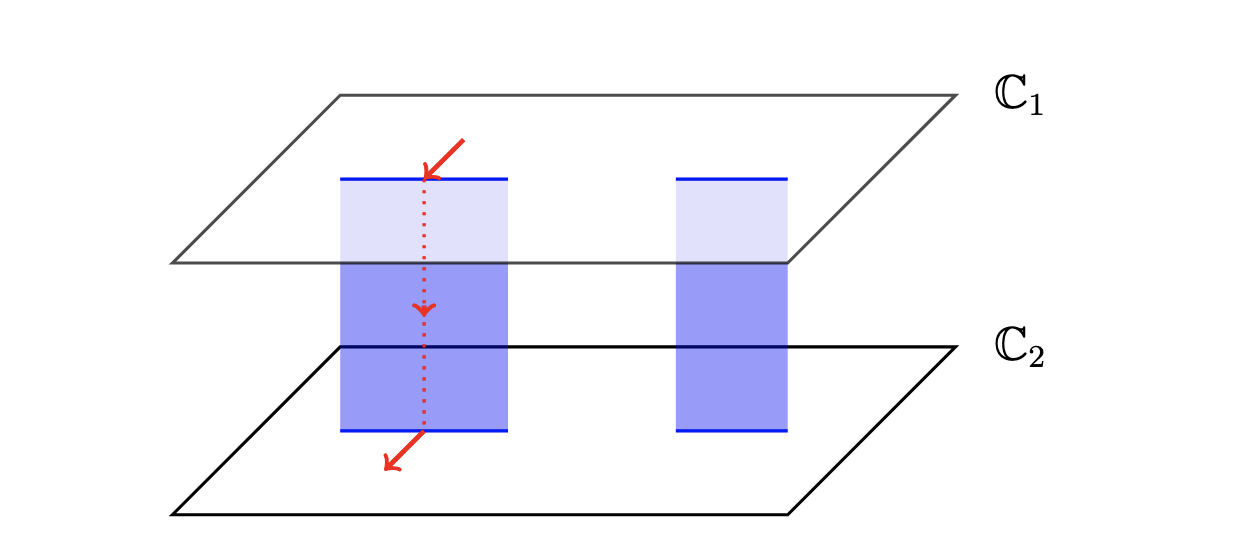
\includegraphics[width=0.45\textwidth]{assets/ghadshi.png}
  \caption{Riemann Surface of the Resolvent}
  \label{fig:ghadshi}
\end{figure}
Thus, if we consider the density of states are non-zero on two separate intervals on the real line, then we have two branch cuts on the real line. Thus the Riemann surface defined has the topology of a torues (if we compactify the complex plane to a sphere). 
\begin{figure}[H]
  \centering
  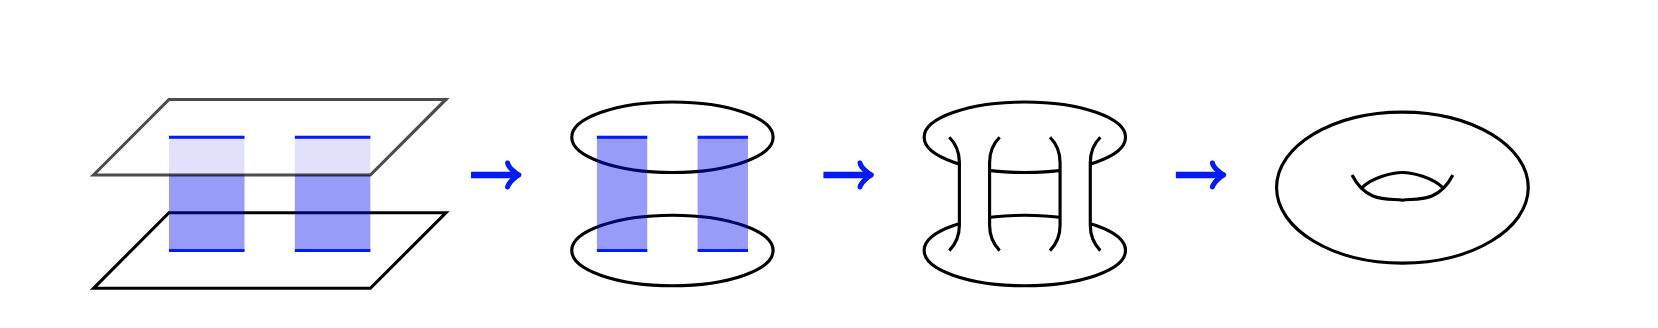
\includegraphics[width=0.8\textwidth]{assets/torus.png}
  \caption{Torus defined by two branch cuts on the real line}
  \label{fig:torus}
\end{figure}
In fact we have a general formula for the genus of the Riemann surface defined by the resolvent. If the there is $ s $ cuts on the real line, then the genus of the Riemann surface defined is:
\begin{align}
  g = s - 1
\end{align}



\subsubsection{Spectral Curve}


\subsection{Preparation for Aymptotic Expansion}

\YL{[Stuffs like the 4point function]}
